\chapter{Resultados}
\label{sec:Resultados}

Para a validação do método proposto neste trabalho, foram realizados dois experimentos baseados no Projeto \textit{Paracoccidioides brasilienses} Genoma do (Projeto Genoma Pb) e no Projeto Genoma Guaraná. Ambos os experimentos foram executados tanto para validar o funcionamento do sistema quanto para verificar a acurácia da ferramenta.


A Figura \ref{sec:TelaConfig} mostra a tela inicial e as ferramentas e bancos de dados já instalados no ncRNA-Agents.

\begin{figure}[htb!] \label{sec:TelaConfig}
\centering
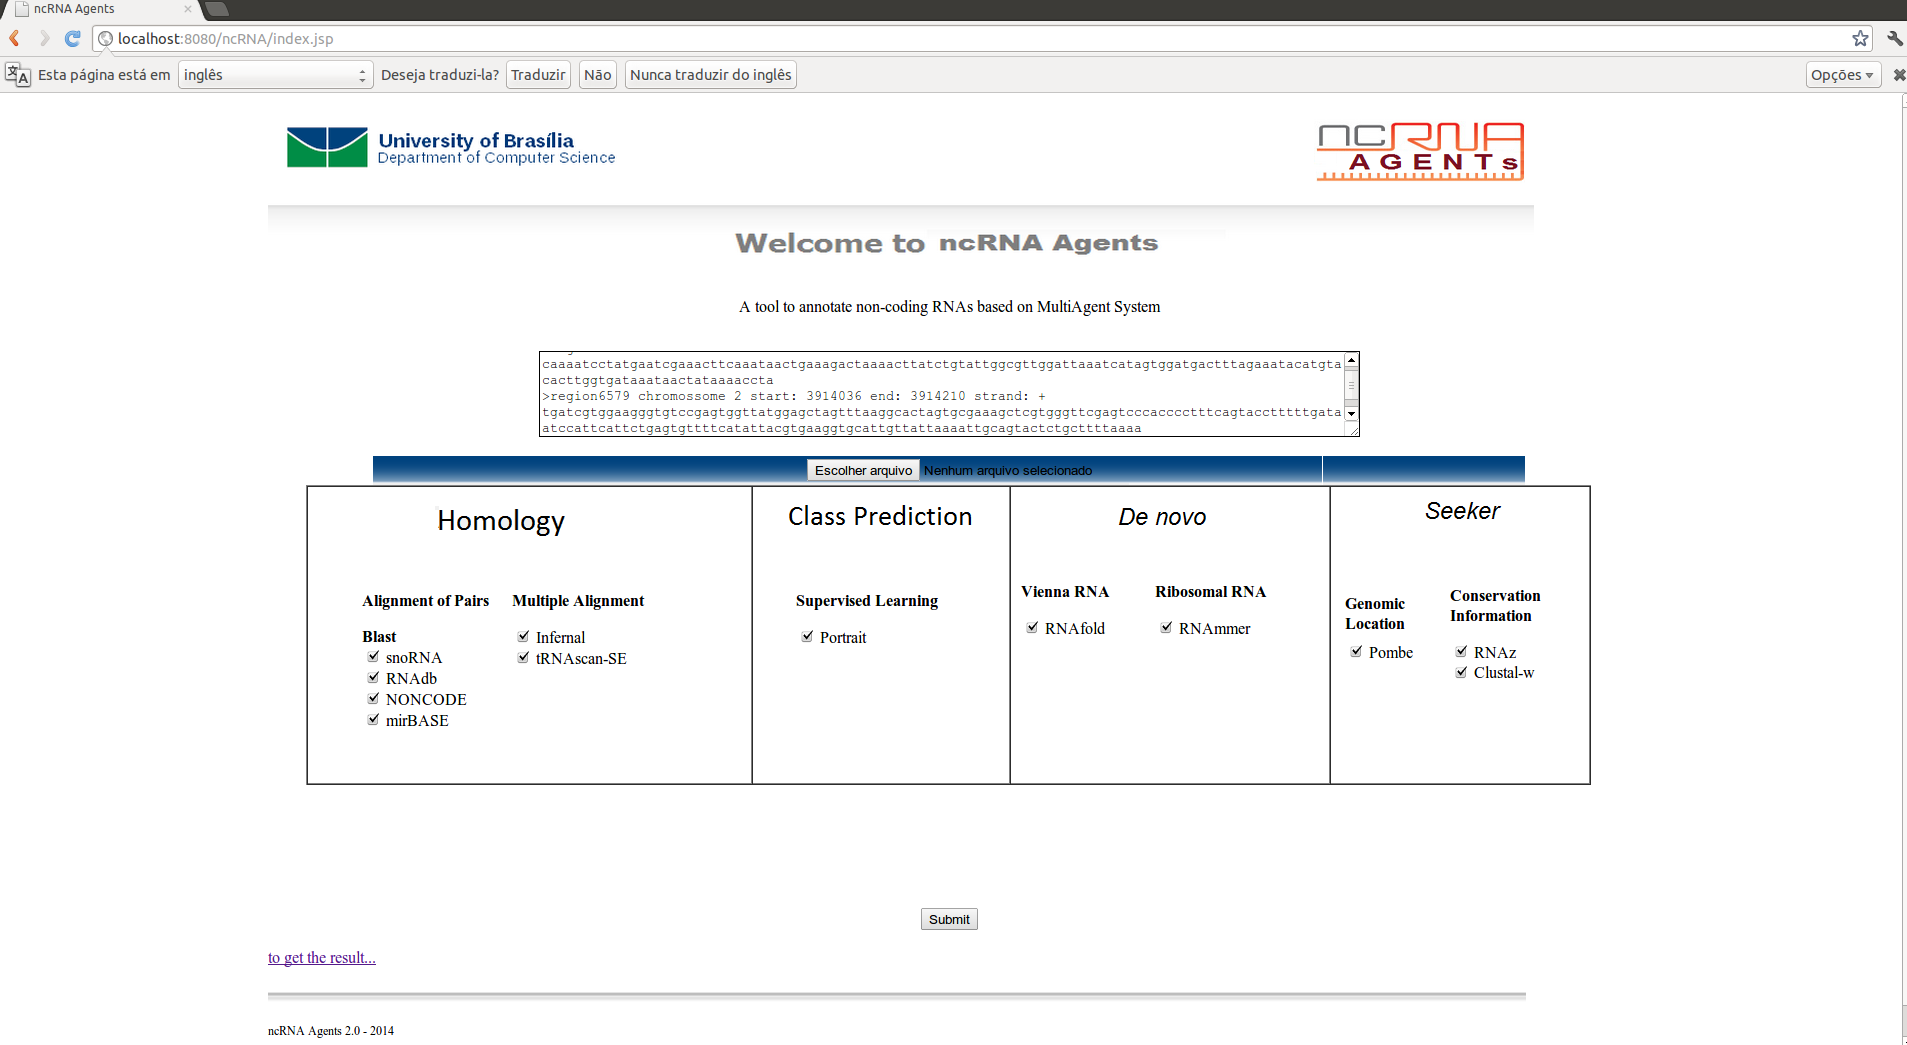
\includegraphics[angle=0,width=1.0\textwidth]{imagens//TelaConfig.png}
\caption{Página do ncRNA-Agents, mostrando as ferramentas e os bancos de dados usados nos experimentos. \label{sec:TelaConfig}}
\end{figure}

A Figura \ref{sec:TelaRespostaInfernal} e \ref{sec:TelaFinalExec} mostram \textit{screenshots} de \textit{sniffers} para visualização do comportamento dos agentes do ncRNA-Agents

\begin{figure}[htb!]
\centering
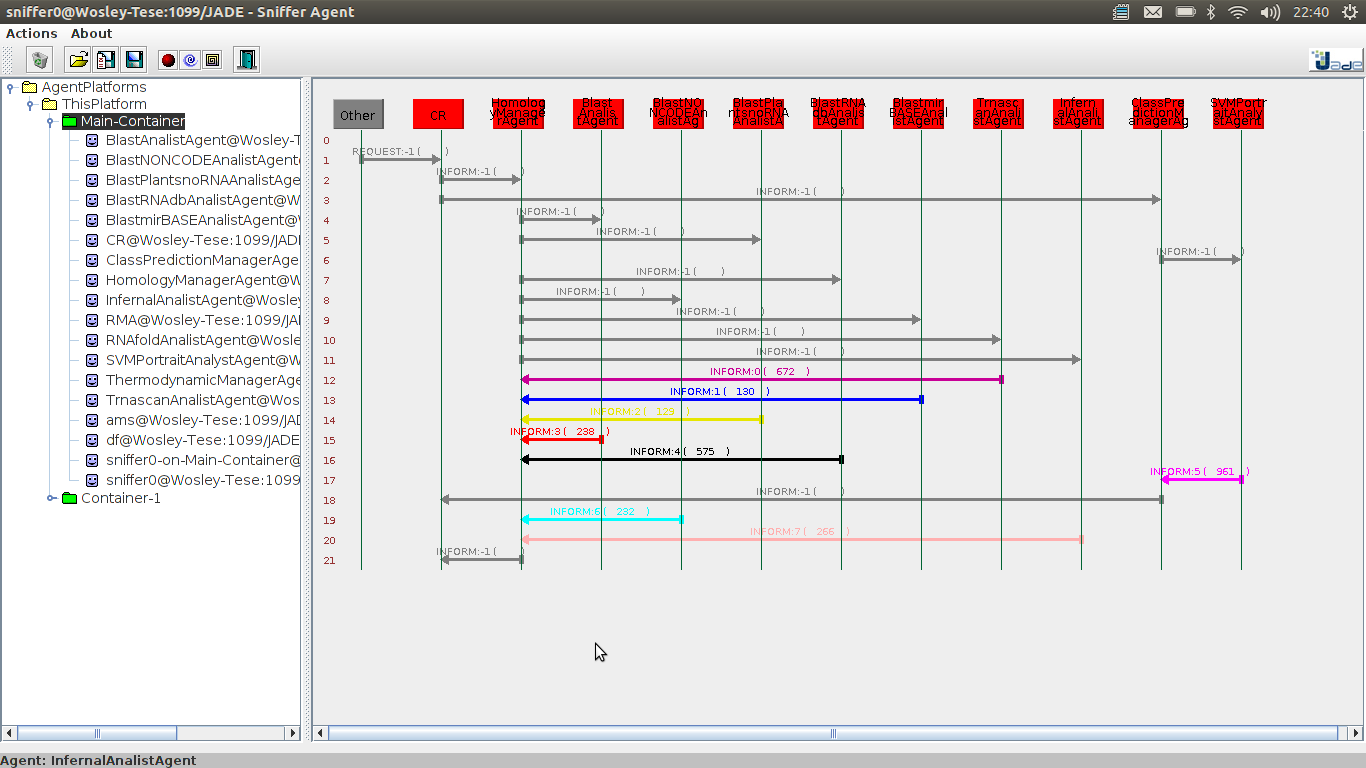
\includegraphics[angle=0,width=0.8\textwidth]{imagens//RespostaInferanal.png}
\caption{\textit{Sniffer} dos agentes do ncRNA-Agents: Aguardando tomada de decisão da camada RC.\label{sec:TelaRespostaInfernal}}
\end{figure}


\begin{figure}[htb!]
\centering
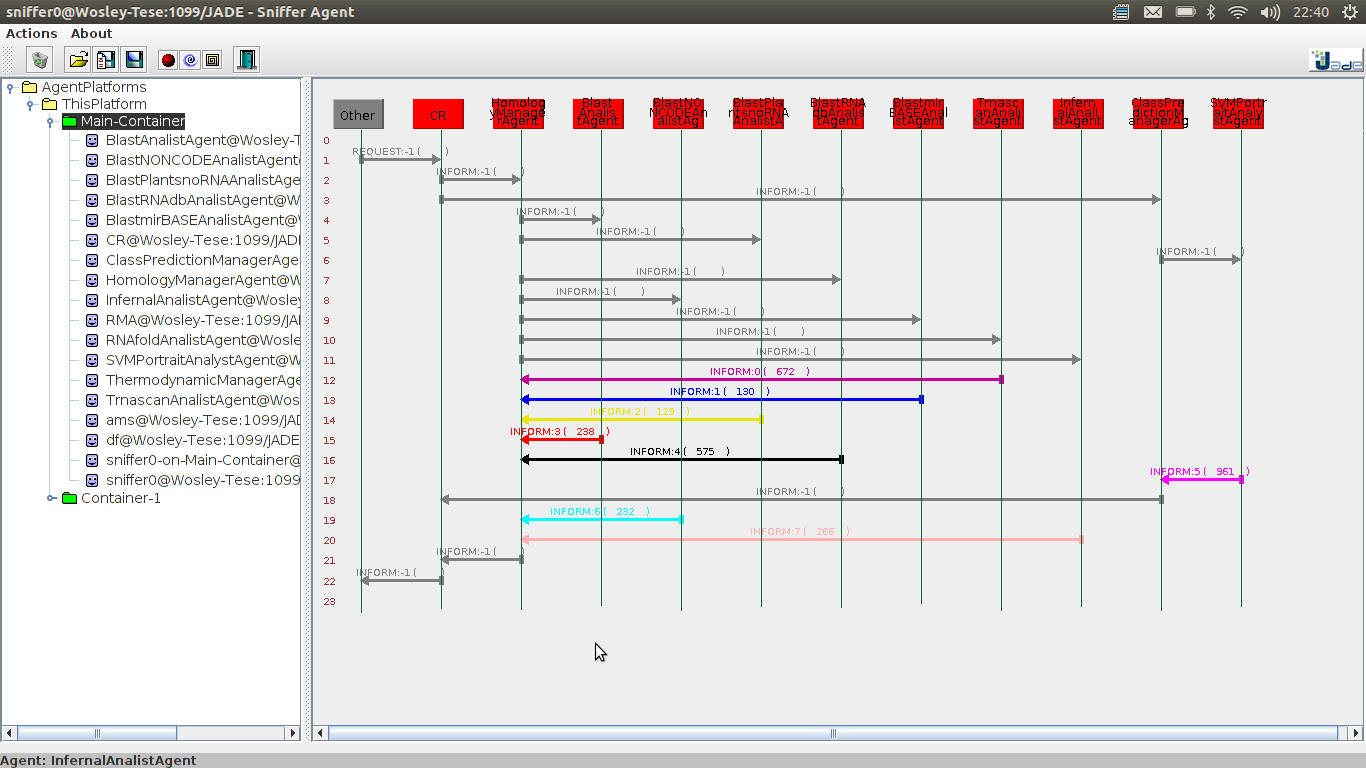
\includegraphics[angle=0,width=0.8\textwidth]{imagens//FinalExe.png}
\caption{\textit{Sniffer} dos agentes do ncRNA-Agents: Enviando resposta para a interface.\label{sec:TelaFinalExec}}
\end{figure}


\newpage
\subsection{Obtidos} \label{sec:Resulobtidos}

Os estudos de caso foram conduzidos para identificar ncRNAs em dois projetos transcritoma: Projeto Genoma Pb e Projeto Genoma Guaraná. No primeiro, foram utilizados: o BLAST com os bancos de dados snoRNA, RNAdb, NONCODE, mirBASE, Infernal e o banco de Rfam 10,1, trRNAscan-SE e SVM-Portrait. No Projeto Genoma Guaraná, foram usados esses mesmos bancos, além do banco de dados Plant-snoRNA.

Esses estudos foram feitos utilizando 200 sequências de cada projeto, buscando a identificação de ncRNAs, observando-se que ainda não foram identificados ncRNAs nos dois projetos. As Tabelas (\ref{fig:ResulProjPb}) e (\ref{fig:ResulProjGuarana}) mostram os resultados obtidos.

\begin{table}[htb!]
\caption{ncRNAs identificados no Projeto Genoma Pb.} \label{fig:ResulProjPb}
\centering
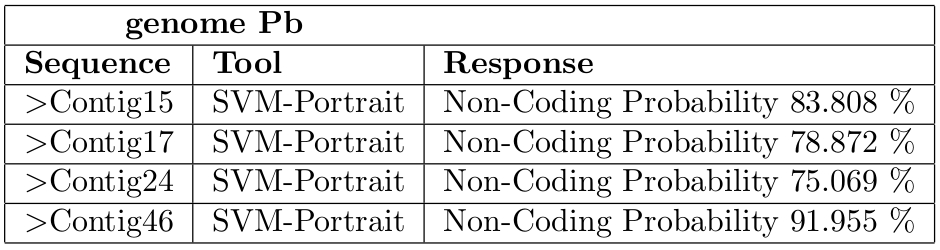
\includegraphics[angle=0,width=0.8\textwidth]{imagens//fig2.JPEG} %\label{fig:AcidosNucleicos}}
\end{table}


\begin{table}[htb!]
\caption{ncRNAs identificados no Projeto Genoma Guaraná.} \label{fig:ResulProjGuarana}
\centering
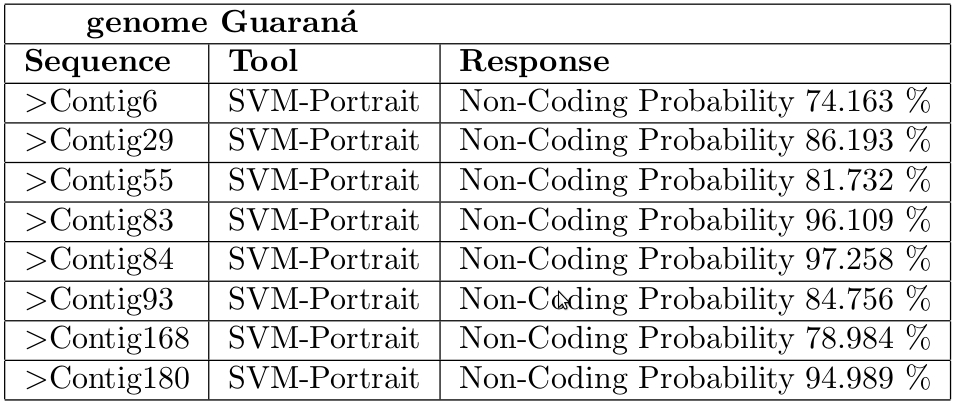
\includegraphics[angle=0,width=0.8\textwidth]{imagens//fig1.JPEG}
\end{table}


\subsubsection{P. brasiliensis} \label{sec:PBrasili}


\subsubsection{P. pombe} \label{sec:SPombe}



%Os testes nos dois projetos serão extendidos para todas as sequências dos dois Projetos Genoma, Pb (6.022) sequências e Guaraná com (8.000).
%
%Será disponibilizado o sistema pela web.
%
%Serão realizados mais experimentos com outros Projetos Genoma.
%
%
%
